\documentclass{beamer}
\usetheme{metropolis}
\usepackage[utf8]{inputenc}
\usepackage[T1]{fontenc}
\usepackage[french]{babel}
\usepackage{blindtext}
\usepackage{listings}
\usepackage{graphicx}
\usepackage{hyperref}
\usepackage{xcolor}
\usepackage{svg}
\usepackage{tikz}
\usepackage{outlines}
\usepackage{pifont}
\usepackage{amsmath}
\usepackage{minted}
\usepackage{changepage}

\usetikzlibrary{positioning, arrows.meta, decorations.markings}
% Define custom colors
\definecolor{commentgray}{rgb}{0.5, 0.5, 0.5}
\definecolor{keywordorange}{rgb}{0.8, 0.4, 0.0}
\definecolor{typeblue}{rgb}{0.2, 0.6, 1.0}
\definecolor{fggray}{rgb}{0.4, 0.4, 0.4}

\makeatletter
\newlength\beamerleftmargin
\setlength\beamerleftmargin{\Gm@lmargin}
\makeatother

% \AtBeginSection[]
% {
%   \begin{frame}
%     \frametitle{Table of Contents}
%     \tableofcontents[currentsection]
%   \end{frame}
% }

\title{Fearless and blazingly fast async HDLC}
\author{Etienne Collin, Emeric Laberge}
\date{\today}

\begin{document}

\maketitle

\begin{frame}{Plan de la présentation}
	\begin{minipage}[c]{0.6\textwidth}
		\vfill
		\tableofcontents
		\vfill
	\end{minipage}%
	\hfill
	\begin{minipage}[c]{0.4\textwidth}
		\vfill
		
\includegraphics[width=0.2\paperwidth]{rust.png}
		\vfill
	\end{minipage}
\end{frame}

\section{Architecture}
\begin{frame}{Architecture du Projet}
	\begin{itemize}
		\item Client
		      \begin{itemize}
			      \item Reader
			      \item Writer
			      \item Send File
		      \end{itemize}
		\item Server
		      \begin{itemize}
			      \item Reader
			      \item Writer
			      \item Assembler
		      \end{itemize}
		\item Tunnel?
	\end{itemize}
\end{frame}

\begin{frame}{Architecture sans Tunnel}
	\begin{tikzpicture}[scale=0.5, node distance=4cm]
		% Nodes
		\node (client) [draw, rectangle] {Client};
		\node (writer_c) [draw, rectangle, above right of=client]{Writer};
		\node (reader_c) [draw, rectangle, below right of=client]{Reader};
		\node (writer_s) [draw, rectangle, right of=reader_c]{Writer};
		\node (reader_s) [draw, rectangle,  right of=writer_c]{Reader};
		\node (server) [draw, rectangle, below right of=reader_s]{Serveur};
		\node[right of=client, xshift=1cm] (lost) [draw, rectangle,dashed]{Trame perdue};

		% font size to small
		\tiny

		% Arrows
		% Lost frame annotation
		\path[->] (client) edge[bend left=45] node[fill=white] {Envoie de
				trame}(writer_c.west);
		\path[->] (writer_c) edge node[fill=white, align=center]{Probabilité de\\bit flip} (reader_s.west);
		\path[->] (reader_s.east) edge[bend left=45] node[fill=white]{Réception de trame} (server);
		\path[->] (writer_s) edge node[fill=white, align=center]{Probabilité de\\bit flip} (reader_c.east);
		\path[->] (reader_c.west) edge[bend left=45] node[fill=white]{Réception de trame} (client);
		\path[->] (server) edge[bend left=45] node[fill=white] {Envoie de
				trame}(writer_s.east);


		\path[dashed,->] (writer_c) edge node[fill=white] {Perte de trame} (lost);
		\path[dashed,->] (writer_s) edge node[fill=white] {Perte de trame} (lost);

	\end{tikzpicture}
\end{frame}

\begin{frame}{Architecture avec Tunnel}
	\begin{tikzpicture}[scale=0.8, node distance=4cm]
		% Nodes
		\node (client) [draw, rectangle] {Client};
		\node (tunnel) [draw, rectangle, right of=client] {Tunnel};
		\node (server) [draw, rectangle, right of=tunnel] {Serveur};
		\node[below of=tunnel, yshift=2cm] (lost) [draw, rectangle,dashed]{Trame perdue};

		% font size to small
		\tiny

		% Arrows
		% Lost frame annotation
		\path[->] (client.north east) edge[bend left=45] node[fill=white] {Envoie de
				trame}(tunnel.north west);
		\path[->] (tunnel.north east) edge[bend left=45] node[fill=white] {Réception
				de trame}(server.north west);
		\path[->] (server.south west) edge[bend left=45] node[fill=white]
			{Envoie de trame}(tunnel.south east);
		\path[->] (tunnel.south west) edge[bend left=45] node[fill=white] {Réception
				de trame}(client.south east);
		\path[dashed,->] (tunnel) edge[] node[fill=white] {Perte de trame} (lost);
		\draw[dashed,->] (tunnel) [loop above] to node {Bit flip} (tunnel);
		\path[->] (server) edge[loop right] node {ACK}(server);
	\end{tikzpicture}
\end{frame}

\begin{frame}{Visualisation détaillée de l'architecture}
	\hspace{-\beamerleftmargin}%
	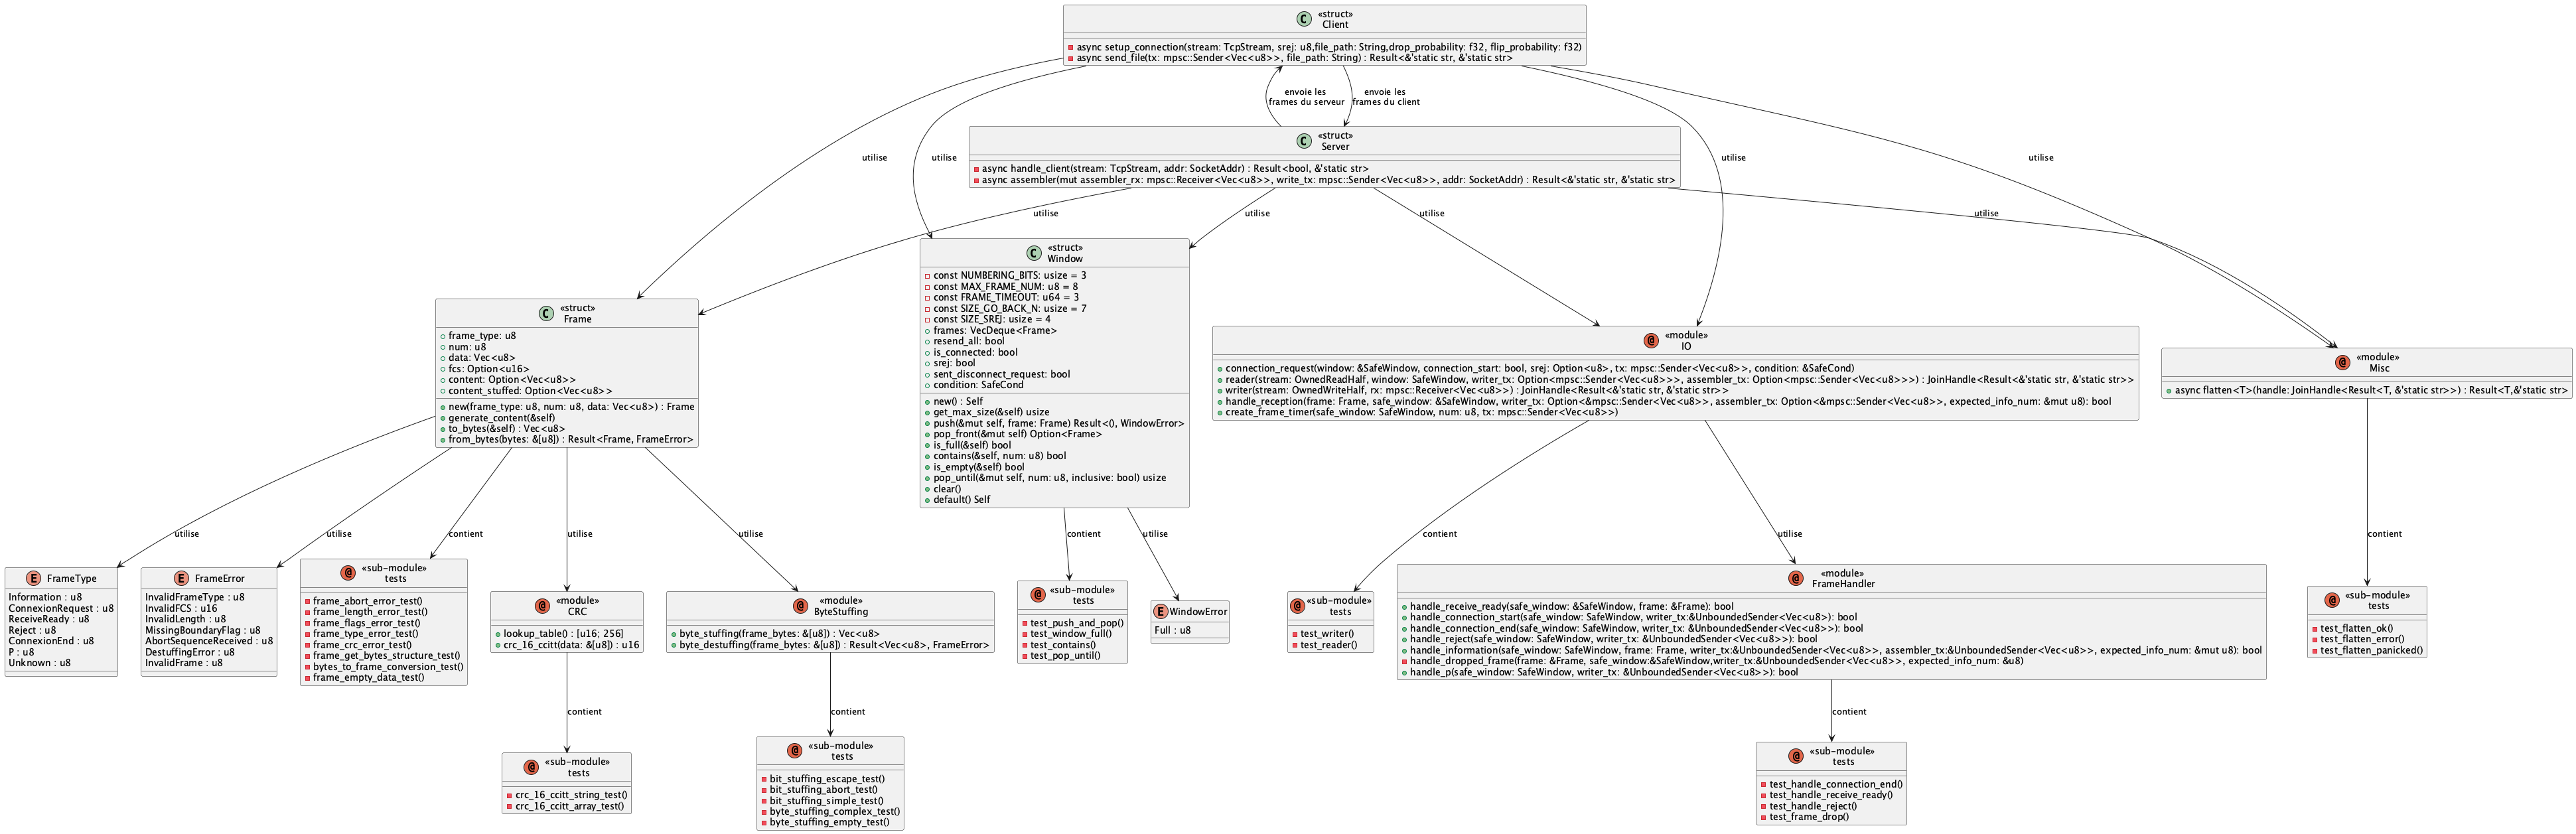
\includegraphics[width=\paperwidth]{class-diagram.png}
\end{frame}

\section{Implémentation}
\begin{frame}{Implémentation}
	\begin{itemize}
		\item Rust
		      \begin{itemize}
			      \item Memory Safe (même sans GC)
			      \item Press Release: Future Software Should Be Memory Safe
			      \item FAANG, Microsoft, Linux, NSA
		      \end{itemize}
		\item Design Asynchrone
		      \begin{itemize}
			      \item Synchronisation
			      \item MPSC (Multi-Producer Single Consumer)
			      \item Thread Safe
		      \end{itemize}
		\item Utilisation directe des bytes
		      \begin{itemize}
			      \item Versus string (espace x8-x32)
		      \end{itemize}
	\end{itemize}
\end{frame}

\section{Client}
\begin{frame}{Fonctionnalités du client}
	\begin{itemize}
		\item Établissement de la connexion
		\item Séparation des données en trames
		\item Utilisation des utils
		\item Gestion de la fenêtre d'envoi
		\item Fermeture de la connexion
	\end{itemize}
\end{frame}

\begin{frame}{Séparation des données en trames}
	Voici le format des trames que nous avons utilisé :
	$$
		\begin{tabular}{|c|c|c|c|c|c|c|c|c|c|c|c|}
			\hline
			\textbf{Flag} & \textbf{Type} & \textbf{Num} & \textbf{Données} &
			\textbf{CRC}  & \textbf{Flag}                                                        \\
			1 octet       & 1 octet       & 1 octet      & 1 à 64Ko         & 2 octets & 1 octet \\
			\hline
		\end{tabular}
	$$

	{\small
			Il est important de noter que les données ajoutées par le byte stuffing sont
			incluses dans le champ données.\\

		}
	\centerline{
		\rule{0.8\textwidth}{0.2pt}
	}

	\textbf{Scénario :}\\
	Taille des données à envoyer : 128Ko \\
	Taille des données après byte stuffing : 140Ko
	\begin{enumerate}
		\item Première trame : contient les 64 premiers Ko
		\item Deuxième trame : contient les 64 Ko suivants
		\item Troisième trame : contient les 12 Ko restants
	\end{enumerate}
\end{frame}


\section{Server}
\begin{frame}{Fonctionnalités du Récepteur}
	Les fonctionnalités du récepteur sont les suivantes :
	\begin{itemize}
		\item Établissement de la connexion
		\item Utilisation des utils
		\item Assemblage des trames reçues
		\item Fermeture de la connexion
	\end{itemize}
\end{frame}

\section{Utils}
\begin{frame}{Utils}
	Design modulaire!
\end{frame}

\begin{frame}{Fonctionnalités}
	\begin{itemize}
		\item Gestion des trames
		      \begin{itemize}
			      \item Création
			      \item Conversion bytes $\rightarrow$ trame
			            \begin{itemize}
				            \item Vérification intégrité
			            \end{itemize}
			      \item Conversion trame $\rightarrow$ bytes
			            \begin{itemize}
				            \item Calcul CRC et byte stuffing
			            \end{itemize}
		      \end{itemize}
		\item Gestion de la fenêtre
		      \begin{itemize}
			      \item Création
			      \item Push \& Pop
			      \item Temporisateurs async
			      \item Condvar
		      \end{itemize}
	\end{itemize}
\end{frame}

\begin{frame}{Fonctionnalités}
	\begin{itemize}
		\item Envoi des trames
		      \begin{itemize}
			      \item Byte stuffing
			      \item Byte destuffing
			      \item Attente de l'acquittement
			      \item Trames perdues
			      \item Trames corrompues
		      \end{itemize}
		\item Réception et traitement des trames
		      \begin{itemize}
			      \item Vérification de l'intégrité des données
			      \item Gestion des erreurs ou des pertes de trames
			      \item Gestion de la fenêtre de réception
			      \item Envoi d'acquittements
		      \end{itemize}
	\end{itemize}
\end{frame}

\begin{frame}{Gestion de la fenêtre de réception}
	\begin{outline}
		\1 $\texttt{NUMBERING\_BITS}$: Nombre de bits pour numéroter les trames
		\2[\ding{43}] $\texttt{NUMBERING\_BITS} \rightarrow 3$
		\1 $\texttt{MAX\_FRAME\_NUM}$: Valeur maximale du numéro d'une trame
		\2[\ding{43}] $\texttt{MAX\_FRAME\_NUM} \rightarrow $ 1 $\vcenter{\hbox{<<}}$
		$\texttt{NUMBERING\_BITS}$ ou $2^{\texttt{NUMBERING\_BITS}}$
		\1 $\texttt{SIZE\_GO\_BACK\_N}$: Taille maximale de la fenêtre pour le protocole
		Go-Back-N
		\2[\ding{43}] $\texttt{SIZE\_GO\_BACK\_N} \rightarrow$ (1 $\vcenter{\hbox{<<}}$
		$\texttt{NUMBERING\_BITS}) - 1$
	\end{outline}
\end{frame}

\section{CRC}
\begin{frame}{Implémentation}
	\begin{itemize}
		\item LUT
		      \begin{itemize}
			      \item Systèmes embarqués
			      \item Rapide!!!
			      \item Taille en mémoire 16x16
		      \end{itemize}
	\end{itemize}
\end{frame}


\begin{frame}[fragile]{Implémentation du CRC}

	{\scriptsize
		\begin{minted}{Rust}
/// CRC-16 CCITT implementation.
/// This function computes the CRC-16 CCITT checksum for the given data.
pub fn crc_16_ccitt(data: &[u8]) -> PolynomialSize {
    let mut remainder = INITIAL_VALUE;
    // For each byte in the data, find its corresponding value 
    // in the lookup table and XOR it with the remainder.
    // Then, shift the remainder 8 bits to the left.
    data.iter().for_each(|byte| {
        // Isolate the upper byte of the current remainder
        let processed_byte = *byte ^ (remainder >> (POLYNOM_WIDTH - 8)) as u8;
        // XOR the remainder with the value from the lookup table
        remainder = LUT[processed_byte as usize] ^ (remainder << 8);
    });
    remainder ^ FINAL_XOR
}
\end{minted}
	}

\end{frame}

\begin{frame}{Problème du bit stuffing}
	$$
		\begin{tabular}{|c|c|}
			\hline
			$\textbf{11111100}$ & $\textbf{10110011}$ \\
			\hline
		\end{tabular}
		\vspace{-6pt}
	$$
	\begin{center}
		$\downarrow$
	\end{center}
	\vspace{-6pt}
	$$
		\begin{tabular}{|c|c|c|}
			\hline
			$\textbf{11111}{\color{red}0}\textbf{10}$ & $\textbf{01011001}$ & $\textbf{1}$0000000 \\
			\hline
		\end{tabular}
	$$
	\textbf{On ne sait pas quels bits sont ajoutés comme padding (sans modifier la structure de la trame)!}
\end{frame}

\begin{frame}{Comment byte stuffing règle cela}

	{\scriptsize
		\begin{itemize}
			\item \texttt{ESCAPE\_FLAG} $\rightarrow$ \textbf{0x7D}
			\item \texttt{BOUNDARY\_FLAG} $\rightarrow$ \textbf{0x7E}
			\item \texttt{REPLACEMENT\_BYTE} $\rightarrow$ \textbf{0x20}
		\end{itemize}
		$$
			\begin{tabular}{|c|c|}
				\hline
				\textbf{bits}                       & \textbf{bytes}      \\
				\hline
				10011011 01111101 01001010 01111110 & 0x9B 0x7D 0x4A 0x7E \\
				\hline
			\end{tabular}
			\vspace{-8pt}
		$$
	}

	\textbf{Byte stuffing:}
	{\scriptsize
		\bgroup
		\setlength{\tabcolsep}{0.2em}
		$$
			\begin{tabular}{|c|ccccc|}
				\hline
				\textbf{bytes}          & \multicolumn{5}{c|}{\textbf{bytes après
				stuffing}}                                                                       \\
				\hline
				\texttt{ESCAPE\_FLAG}   & \texttt{ESCAPE\_FLAG}                   & \text{\quad}
				                        & \texttt{ESCAPE\_FLAG}                   & \oplus
				                        & \texttt{REPLACEMENT\_BYTE}                             \\
				\texttt{BOUNDARY\_FLAG} & \texttt{ESCAPE\_FLAG}                   & \text{\quad}
				                        & \texttt{BOUNDARY\_FLAG}                 & \oplus
				                        & \texttt{REPLACEMENT\_BYTE}                             \\
				\hline
			\end{tabular}
			\vspace{-12pt}
		$$
		\egroup


	}
	$$
		\begin{tabular}{|c|c|c|c|}
			\hline
			0x9B & 0x7D & 0x4A & 0x7E \\
			\hline
		\end{tabular}
	$$
	\begin{center}
		\vspace{-8pt}\\
		$\downarrow$\\
		\vspace{-8pt}
	\end{center}
	$$
		\begin{tabular}{|c|c|c|c|c|c|}
			\hline
			0x9B & ${\color{red}\text{0x7D}}$ & $\textbf{0x5D}$ & 0x4A & ${\color{red}\text{0x7D}}$ & $\textbf{0x5E}$
			\\
			\hline
		\end{tabular}
	$$
	\begin{center}
		\vspace{-8pt}\\
		$\downarrow$\\
		\vspace{-8pt}
	\end{center}
	$$
		\begin{tabular}{|c|c|c|c|}
			\hline
			0x9B & 0x7D & 0x4A & 0x7E \\
			\hline
		\end{tabular}
	$$
\end{frame}



\section{Conclusion}
\begin{frame}{Conclusion}
	\begin{itemize}
		\item Optimisations
		\item Ajout de fonctionnalités
	\end{itemize}
\end{frame}

\begin{frame}{Questions?}
	\begin{center}
		\Huge Questions ?
	\end{center}

\end{frame}

\end{document}
